\documentclass[tikz,border=7pt]{standalone}
\usepackage{amsmath,amssymb}

\begin{document}
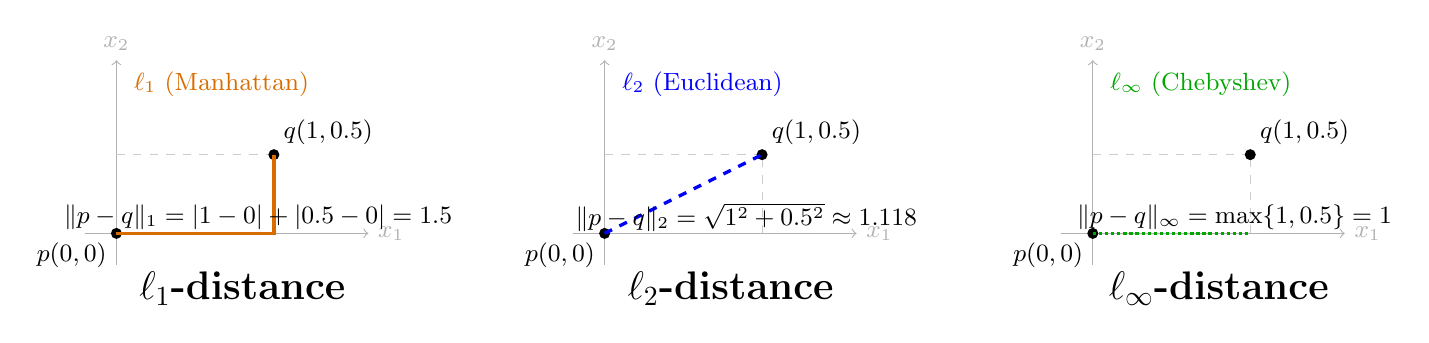
\begin{tikzpicture}[every node/.style={font=\small}]
  %--- common coords
  \def\px{0}\def\py{0}
  \def\qx{1}\def\qy{0.5}

  % helper to draw a small axes box
  \newcommand{\axes}{%
    \draw[->,gray!60] (-0.2,0) -- (1.6,0) node[right] {$x_1$};
    \draw[->,gray!60] (0,-0.2) -- (0,1.1) node[above] {$x_2$};
    \draw[dashed,gray!40] (\qx,0) -- (\qx,\qy);
    \draw[dashed,gray!40] (0,\qy) -- (\qx,\qy);
  }
  % helper to place points
  \newcommand{\points}{%
    \coordinate (p) at (\px,\py);
    \coordinate (q) at (\qx,\qy);
    \fill (p) circle (0.035) node[below left] {$p(0,0)$};
    \fill (q) circle (0.035) node[above right] {$q(1,0.5)$};
  }

  %==================== ℓ1 panel ====================
  \begin{scope}[xshift=0cm, yshift=0cm, scale=2]
    \axes
    \points
    % L1 path (Manhattan): horizontal then vertical
    \draw[very thick,orange!85!black]
      (p) -- (\qx,0) -- (q);
    \node[orange!85!black,anchor=west] at (0.05,0.95) {$\ell_1$ (Manhattan)};
    \node[black] at (0.9,0.1) {$\|p-q\|_1=|1-0|+|0.5-0|=1.5$};
    \node[font=\bfseries] at (0.8,-0.35) {\Large $\ell_1$-distance};
  \end{scope}

  %==================== ℓ2 panel ====================
  \begin{scope}[xshift=6.2cm, yshift=0cm, scale=2]
    \axes
    \points
    % L2 path (Euclidean): straight line
    \draw[very thick,blue,dashed]
      (p) -- (q);
    \node[blue,anchor=west] at (0.05,0.95) {$\ell_2$ (Euclidean)};
    \node[black] at (0.9,0.1) {$\|p-q\|_2=\sqrt{1^2+0.5^2}\approx1.118$};
    \node[font=\bfseries] at (0.8,-0.35) {\Large $\ell_2$-distance};
  \end{scope}

  %==================== ℓ∞ panel ====================
  \begin{scope}[xshift=12.4cm, yshift=0cm, scale=2]
    \axes
    \points
    % L∞ distance = max(|Δx|,|Δy|) = 1, show by horizontal segment
    \draw[very thick,green!65!black,densely dotted]
      (p) -- (\qx,0);
    \node[green!65!black,anchor=west] at (0.05,0.95) {$\ell_\infty$ (Chebyshev)};
    \node[black] at (0.9,0.1) {$\|p-q\|_\infty=\max\{1,0.5\}=1$};
    \node[font=\bfseries] at (0.8,-0.35) {\Large $\ell_\infty$-distance};
  \end{scope}

\end{tikzpicture}
\end{document}
